\documentclass[sigconf,screen]{acmart}

\usepackage{graphicx}
\graphicspath{ {./Images/} }

\settopmatter{printacmref=false} % Removes citation information below abstract
\renewcommand\footnotetextcopyrightpermission[1]{} % removes footnote with conference information in first column
\pagestyle{plain} % removes running headers


%%
%% \BibTeX command to typeset BibTeX logo in the docs
\AtBeginDocument{%
  \providecommand\BibTeX{{%
    \normalfont B\kern-0.5em{\scshape i\kern-0.25em b}\kern-0.8em\TeX}}}


%% These commands are for a PROCEEDINGS abstract or paper.
\acmConference[Data Science for Software Engineering]{Data Science for Software Engineering}{Fall 2020}{Zurich, CH}


%%
%% end of the preamble, start of the body of the document source.
\begin{document}

%%
%% The "title" command has an optional parameter,
%% allowing the author to define a "short title" to be used in page headers.
\title{Reproduction of "Predicting the Severity of a Reported Bug"}

%%
%% The "author" command and its associated commands are used to define
%% the authors and their affiliations.
%% Of note is the shared affiliation of the first two authors, and the
%% "authornote" and "authornotemark" commands
%% used to denote shared contribution to the research.
\author{Andrina Vincenz}
\email{andrina.vincenz@uzh.ch}
\affiliation{%
  \institution{University of Zurich}
  \city{Zurich}
  \country{Switzerland}
}

\author{David Stalder}
\email{david.stalder@uzh.ch}
\affiliation{%
  \institution{University of Zurich}
  \city{Zurich}
  \country{Switzerland}
}


%%
%% By default, the full list of authors will be used in the page
%% headers. Often, this list is too long, and will overlap
%% other information printed in the page headers. This command allows
%% the author to define a more concise list
%% of authors' names for this purpose.
\renewcommand{\shortauthors}{Andrina Vincenz, David Stalder}

%%
%% The abstract is a short summary of the work to be presented in the
%% article.
\begin{abstract}
	
	\textbf{Background.} Bug fixing is a fundamental part of software maintenance. Bugs have different levels of severity according to their threat to the system and urgency to fixing.
	
	\textbf{Aim.} The aim is to have models which are able to identify the severity of bug reports.
	
	\textbf{Method.} After identifying the system, bug reports will be extracted from bugzilla including the severity of the bug. This data is used to train two classifiers: SGDClassifier and Multinomial Na{\"\i}ve Bayes. The following measurements are used to identify the quality of the model: precision, recall and f-measures.
	
	\textbf{Conclusion.} This study will show if it is possible to generate models, which can do the classification of bug reports automatically with certainty. This can help software engineers in practice to classify their bug reports and focus on the most urgent.
\end{abstract}


%%
%% This command processes the author and affiliation and title
%% information and builds the first part of the formatted document.
\maketitle

\section{Introduction}
Bug reports represent a fundamental part of software maintenance by documenting the malfunction of a software part. A large number of bug reports by users and developers are collected on a daily basis in bug tracking systems like Bugzilla. These reports are then manually prioritized according to their severity and classified into 6 groups, ranging from a request to enhancement to a critical level resulting in crashes, loss of data or severe memory leak. The level of severity indicates the impact of the bug on the successful execution of a software system.

However, the manual assignment of the severity level to a bug report takes time and resources. In combination with the increase of daily bug reports the classification introduces a set of challenges such as misclassification of severity or the increase of cost. The ability of the automated severity prediction of bug reports by a tool reduces errors in misclassification and manual work as well as enhance the software quality.

In order to automate the severity predication of bug reports, different classification and information retrieval techniques based on textual descriptions have been used previously. Techniques range from Nearest Neighbours \cite{TianDrone} \cite{LamkanfiMiningAlgo} \cite{ChaturvediBugSeverity}, Na{\"\i}ve Bayes \cite{LamkanfiMiningAlgo} \cite{ChaturvediBugSeverity} to Support Vector Machines \cite{KanwalOMSVM} \cite{LamkanfiMiningAlgo} \cite{ChaturvediBugSeverity}. While some work focuses on automatically analyzing the text of past bug reports and the recommendation of severity labels \cite{TianDrone} \cite{LamkanfiMiningAlgo} \cite{ChaturvediBugSeverity} other work creates a classification-based approach to create a bug priority recommender \cite{KanwalOMSVM}.

For this project, we intend to conduct a reproduction of the paper "Predicting the severity of a reported bug" \cite{ourPaper} by Lamkanfy et al. It was originally written in 2010, which we consider as too old for such a current topic. 

The research goal of this paper was to test if it is possible to predict the severity of a reported bug by analysing its textual description by using a text mining algorithm. They came up with subsidiary research questions which need to be included to find an explanation of their research goal.

\begin{itemize}
	\item Concerning the length of a bug report, the research question was: "Which (text) fields in the bug reports serve as the best prediction basis? The one-line summary which briefly focusses on the problem or the longer full description which includes more detail?" \cite{ourPaper}
	
	\item Concerning the scope of the training period, their research question was: "How many samples must be collected before one can make a reliable predictor?" \cite{ourPaper}
	
	\item Concerning the components their research question was: "Is it better to have a specialized predictor for each component of the software system, or can we combine bug reports over different software components (the so-called "cross- component" approach)?" \cite{ourPaper}
\end{itemize}

At the end of the paper they already analysed those research questions. However, we will base our work on the findings which were made by them as follows:

\begin{itemize}
	\item \textit{Short vs. Long}: They found that there is no difference in the prediction basis between the one-line summary and the full description \cite{ourPaper}. To have a smaller set of samples and to make the procedure as efficient as possible, we decided to use only the one-line summary.
	
	\item \textit{Training Period}: They found that there is nearly no difference in the reliability of the predictor by taking 500, 1000 or 2000 samples \cite{ourPaper}. To be sure that our findings will be as precise as possible, we decided to take 2000 samples.
	
	\item \textit{Per Component vs. Cross Component}: They found that using the cross-component approach the performance improves with an increasing number of samples \cite{ourPaper}. Therefore we decided to use the cross-component approach, since we are already using 2000 samples.
\end{itemize}

The structure of the paper is as follows. In the second section "Methodology" we focus on how we conducted our research and explain every step of the work. In the third section "Results" we present our findings, in the fourth section "Discussion and Limitations" we discuss and interpret the findings and name the limitations of our research.

We conducted the procedure as follows: First we downloaded and processed the data such that we could use it for the further procedure. For each of the six severity types we chose 2000 entries for the training list and 200 entries for the testing list. In the next step we trained the two models (Na{\"\i}ve Bayes and SGD). For measuring purposes we used the scores precision, recall and f1. The parameter optimization was achieved using grid search. In the last step the classifiers were applied on the test set. Our experimental results for the Na{\"\i}ve Bayes were 0.402 for all the scores (precision, recall and f1), for the SGD the experimental results for all the scores were  0.405. Finally, the severity types "trivial" and "critical" had with both methods an accuracy of over 60\% and all the other types had an accuracy of between 30-45\%.

\section{Methodology}
In a first step we downloaded the necessary data from Bugzilla tracking system with bugs regarding the case Firefox. In our approach only one case was selected. Since we choose the cross-component approach all components were selected. To make the analysis clearer, the only resolution type chosen is fixed. This is because fixed bugs were worked on and therefor the label more certain. There are eight types of severities: blocker, critical, major, normal, minor, trivial, enhancement and N/A. The categories enhancement and N/A were dropped, N/A since this label has no meaning regarding the problem statement and enhancement because this class is imbalanced with only 45 entries in total as well as these are user requests for features. In contrast to the original paper we decided to run the models on all severities as labels to find out whether we get a similar accuracy or worse. To make the training and test step more coherent, the test and training set were downloaded separately. The test set contains each 2000 entries for each severity resulting in 12000 entries. For the test set we have 200 entries per severity with 1200 entries in total.

After downloading the data, our approach consists of the following steps.

\begin{enumerate}
	\item \textit{Preprocess bug reports}: Afterwards the data was imported into a Jupyter Notebook. The data was further preprocessed by dropping rows with missing values or labels resulting in a training set with 11962 entries and a test set with 1999 entries. Further the punctuation and special characters were removed from the bug summary. For the preprocessing of the bug summary a pipeline was used transforming the words into ngramms ranging from (1,1) to (1,3). Further the features were transformed into the tfidf measure reflecting the importance of a word in a document. The label encoding was done with the method LabelEncoder() from sklearn.
	\item \textit{Training the classifiers}: With the training set two different classifiers were trained. First the NB and SGD classifier were trained without any parameter optimization. To measure the accuracy of each model we used the following scores: precision, recall and f-measures. The calculation of the measurements was done via cross validation. Parameter optimization for both classifiers was achieved with Grid Search. For Na{\"\i}ve Bayes only ngramm optimization was performed. For the SGD classifier the following parameters additionally were optimized: loss function, regularization, and early stopping. The grid search resulted in a best model for each classifier.
	\item \textit{Applying classifiers on test set} To calculate the accuracy of each classifier the best model was run with the test set and the results visualized with a normalized confusion matrix. 
	
\end{enumerate}

\section{Results}
Table \ref{tab:title} shows the precision, the recall, and the f1-score of the two selected classifiers using the data samples from Mozilla.

The results of the two different classifiers are nearly the same, whereas the precision, the recall and the f1-score are nearly identical and varying between 0.40-0.41.

\begin{center}
	\centering
	\captionof{table}{Scores of the two Classifiers}
	\label{tab:title} 
	\begin{tabular}{ |c|c|c|c| } 
		\hline
		\textbf{Classifier} & \textbf{Precision} & \textbf{Recall} & \textbf{f1} \\
		\hline
		Na{\"\i}ve Bayes & 0.402 & 0.402 & 0.402 \\
		\hline
		SGD & 0.405 & 0.405 & 0.405 \\
		\hline
	\end{tabular}
\end{center}

In the next step we used a grid-search for finding the best model of both classifiers. Figure \ref{fig:confMatNB} is the normalized confusion matrix of the best Na{\"\i}ve Bayes model which has an accuracy score of 0.466,  Figure \ref{fig:confMatSGD} is the normalized confusion matrix of the best SGD model which has an accuracy score of 0.455.

\begin{figure}[h]
	\caption{Relative Confusion Matrix of Na{\"\i}ve Bayes Model}
	\centering
	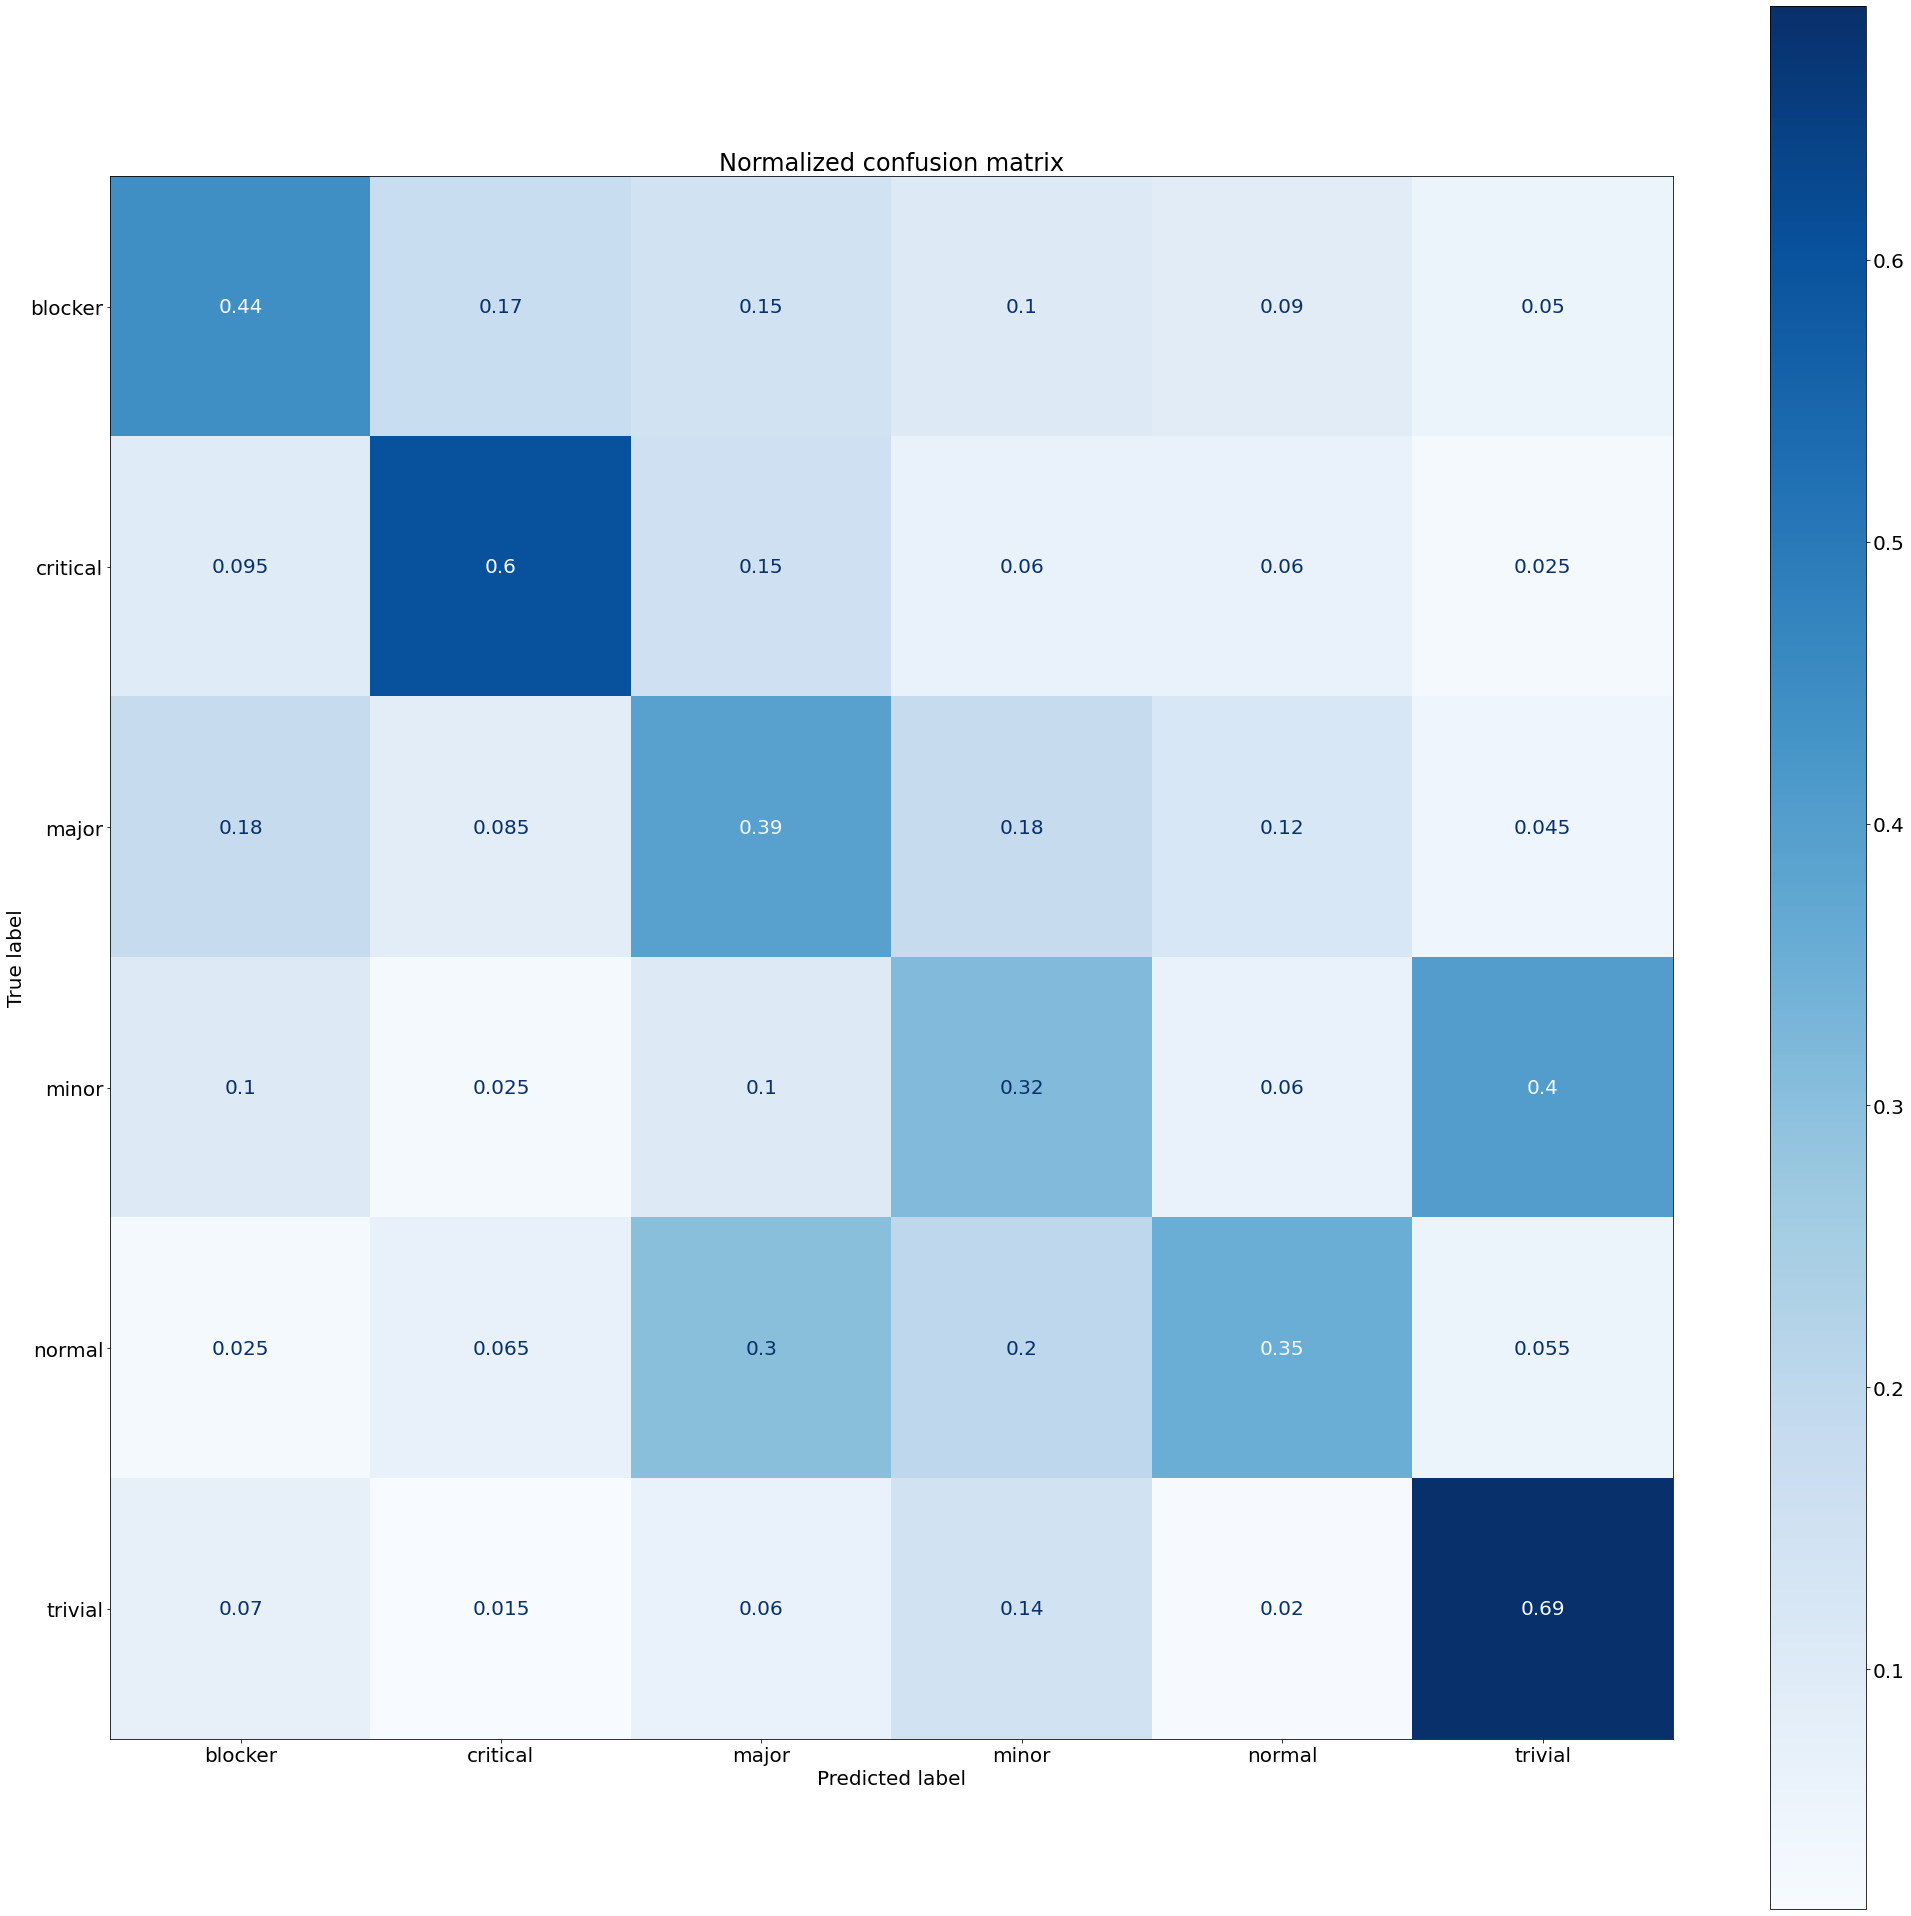
\includegraphics[scale=0.1]{norm_conf_matrix_nb}
	\label{fig:confMatNB}	
\end{figure}

Table \ref{fig:confMatNB} shows the label "blocker" had an accuracy of 0.44, "critical"  0.6, "major" 0.39, "minor" 0.32, "normal" 0.35, and "trivial" 0.69.

\begin{figure}[h]
	\caption{Relative Confusion Matrix of SGD Model}
	\centering
	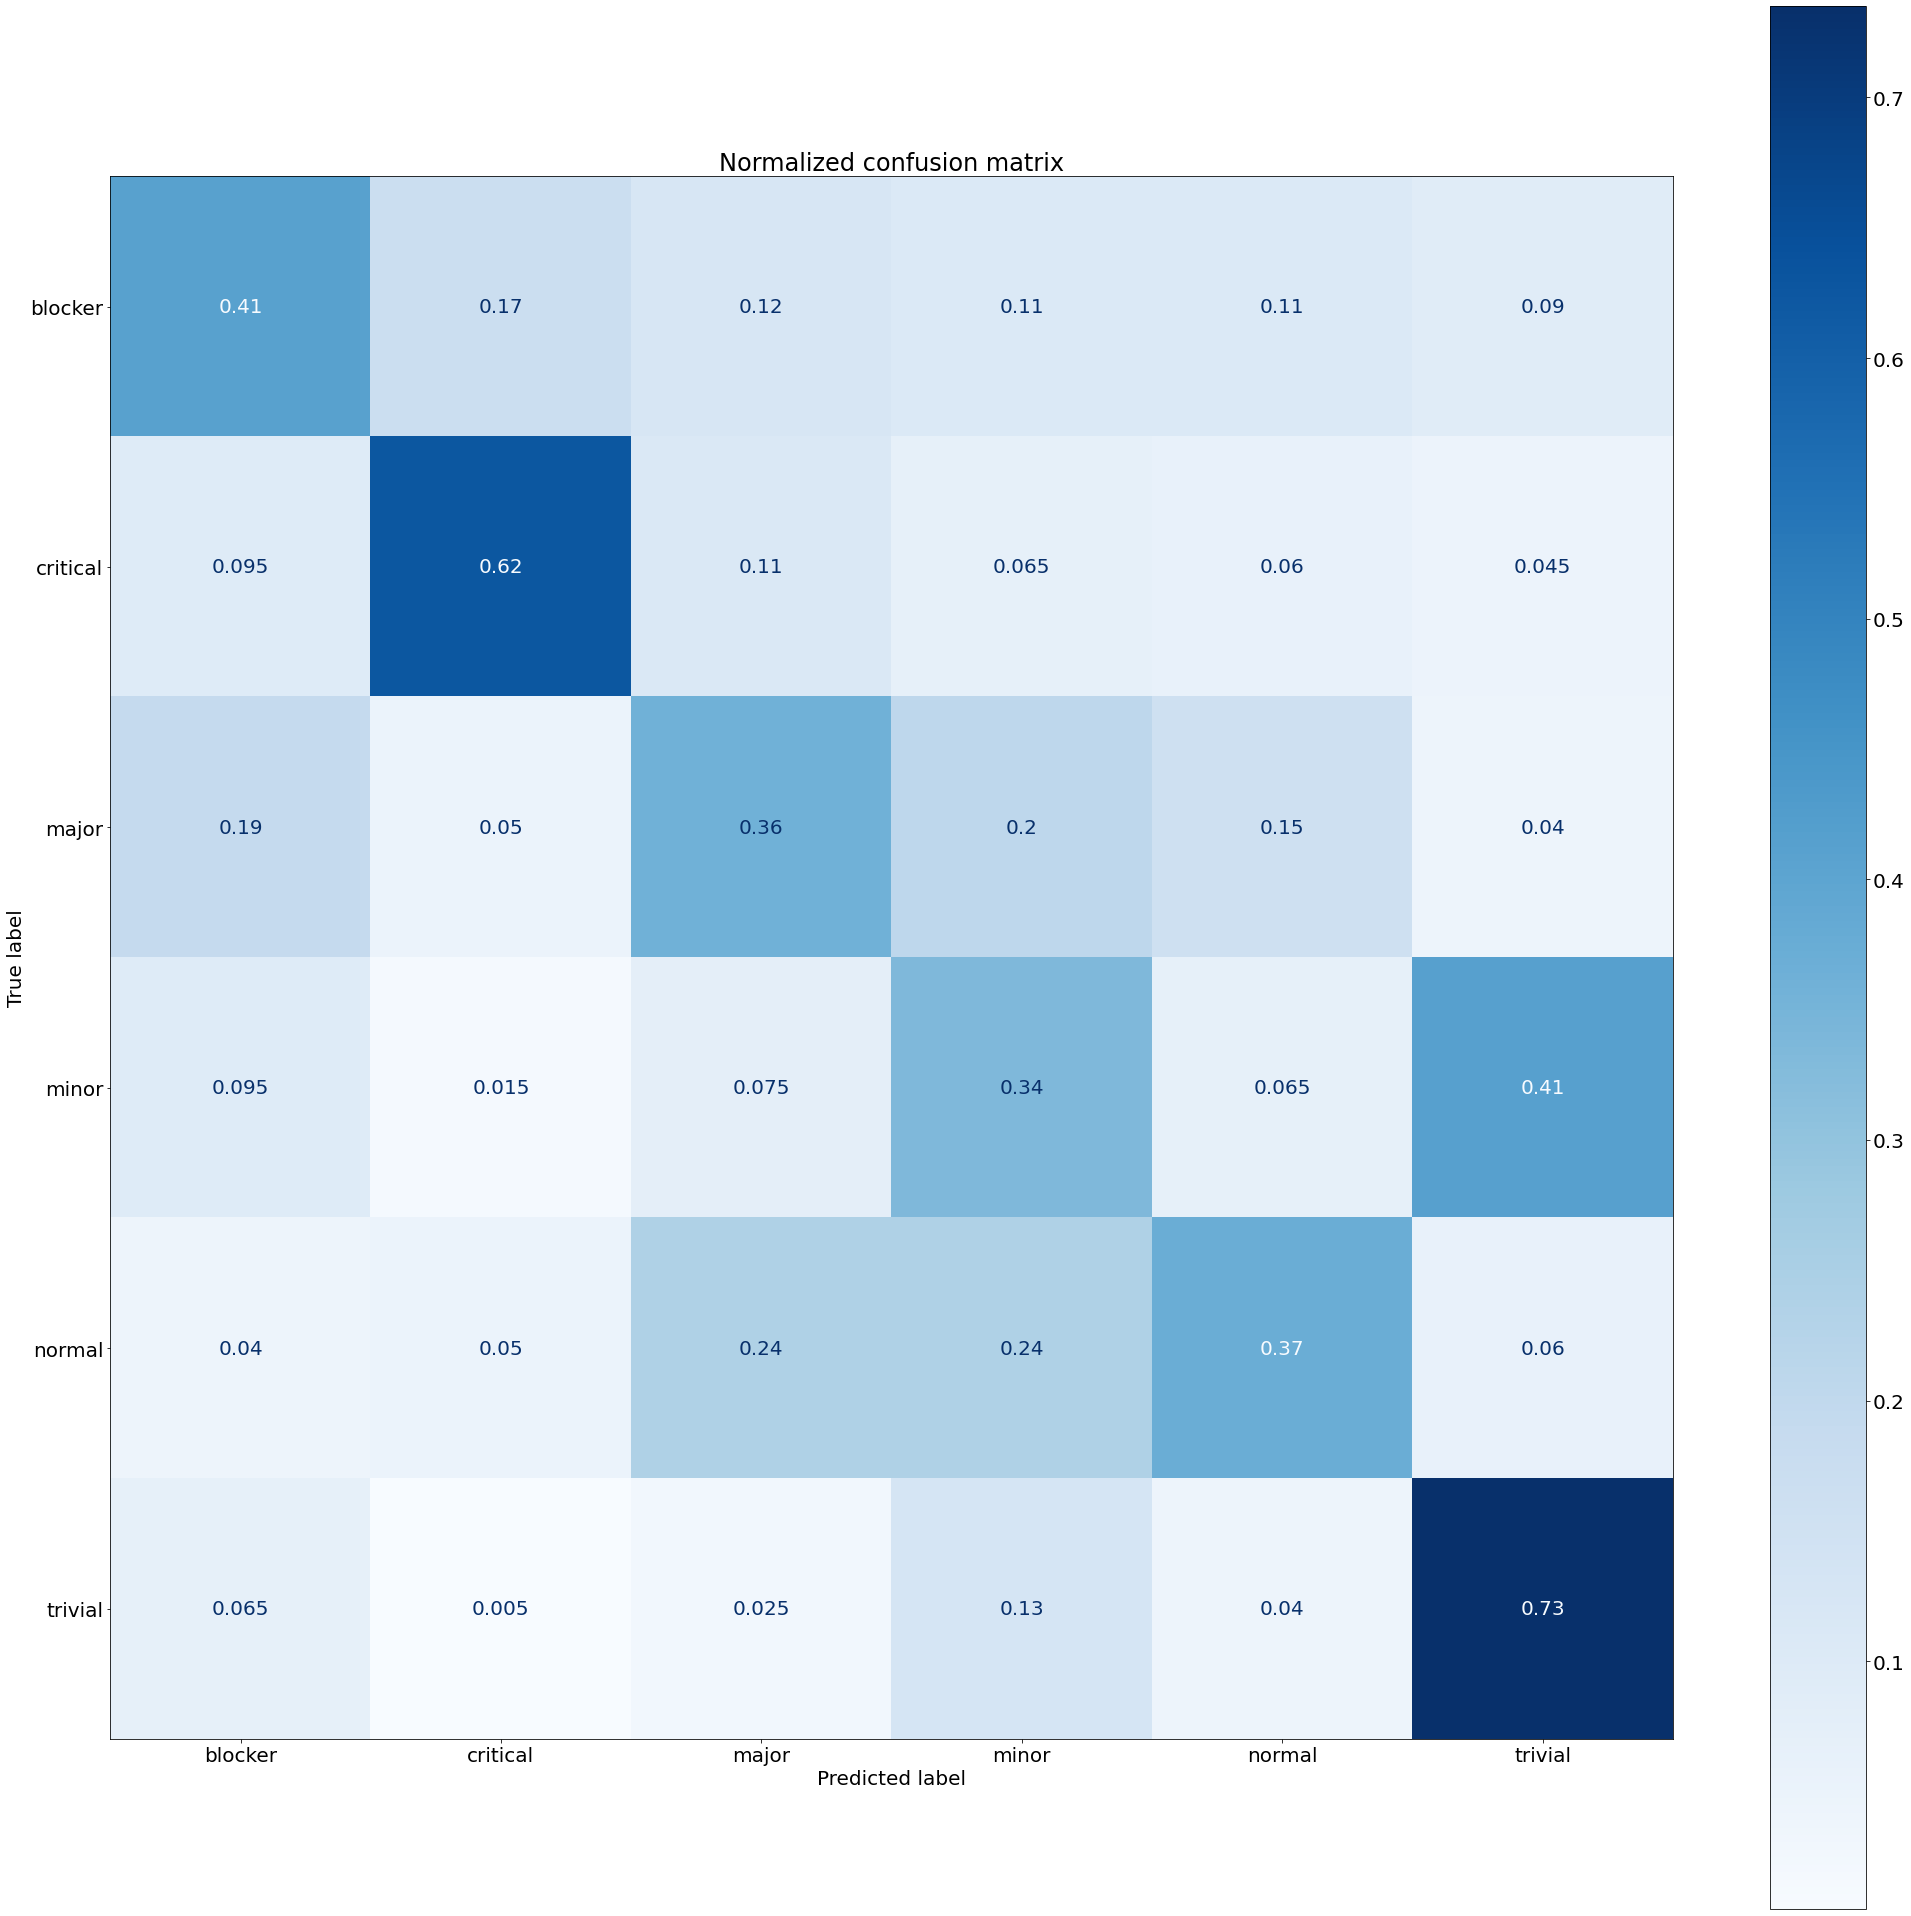
\includegraphics[scale=0.1]{norm_conf_matrix_sgd}
	\label{fig:confMatSGD}	
\end{figure}

Table \ref{fig:confMatSGD} shows the label "blocker" had an accuracy of 0.41, "critical"  0.62, "major" 0.36, "minor" 0.34, "normal" 0.37, and "trivial" 0.73.


\section{Discussion and Limitations}
This approach shows that classifying bugs according to their severity with linear classifiers only works to a certain point. Only two labels were classified with a higher accuracy than 50\%, namely trivial and critical. The reason for this could be that the bug summaries over all components have too similar words to be able to classify them correctly. In this case there is no better solution available with linear models except for larger ngramms. Is this not the case, larger test and trainings files could lead to a higher accuracy for this approach. Compared to the paper \cite{ourPaper} with the same amount of test data for the non-component approach it shows that classifying the bug severity further into two categories leads to a higher accuracy. Training another linear classifier leads to no improvement in accuracy and to similar measurements.

As already mentioned in the section "Results", we observed that in both models the values for precision, recall and f1-score are nearly identical. To be able to find possible explanations, we first need to have a look at the formulae of each score \cite{scoreExplanation}. In the following formulae, TP means "true positive", FP means "false positive", and FN means "false negative".

Precision:
\begin{equation}
	p = \frac{TP}{TP+FP}
	\label{eq:precision}
\end{equation}

Recall:
\begin{equation}
	r = \frac{TP}{TP+FN} = \frac{TP}{TP+FP}
	\label{eq:recall}
\end{equation}

f1:
\begin{equation}
	f1 = \frac{(1+1^2)TP}{(1+1^2)TP +1^2 FN+FP} = \frac{2TP}{2TP+FP+FN} = \frac{TP}{TP+FP}
	\label{eq:f1}
\end{equation}

Since all numbers are nearly the same, in our case we seem to have fp=fn (see in Equations \ref{eq:precision}, \ref{eq:recall}, and \ref{eq:f1}), i.e. the number of false positives must be equal the number of false negatives. This can be interpreted as good, since our data set had an equal amount of each label.


%%
%% The next two lines define the bibliography style to be used, and
%% the bibliography file.
\bibliographystyle{ACM-Reference-Format}
\bibliography{sample-base}

%%
%% If your work has an appendix, this is the place to put it.
\appendix




\end{document}
\endinput
%%
%% End of file `sample-sigconf.tex'.
